\documentclass{article}
\usepackage{amsmath}
\usepackage{pgfplots}
\pgfplotsset{compat=1.16}

\title{\textbf{Assignment 2}}
\author{Abhishek Ajit Sabnis}
\date{24 January 2022}

\begin{document}

\maketitle

\textbf{50) Let X and Y be i.i.d random variables uniformly distributed on (0,4). Then $P(X>Y|X<2Y)$ is}

\vspace{0.5cm}

\textbf{Ans} According to \underline{Bayes Theorem}, for any 2 random variable A and B, 

\begin{equation}
    P(A|B) = \frac{P(A,B)}{P(B)}
\end{equation}

Thus, 

\begin{equation}
    P(X>Y|X<2Y) = \frac{P ((X>Y), (X<2Y)) }{P(X<2Y)}
\end{equation}

\vspace{0.2cm}

\underline{Joint Probability Density Function}

\vspace{0.1cm}

Two random variables A, B are jointly continuous if there exists a function $f_{XY} (x,y)$ such that 

\begin{equation}
    P((X,Y) \in A) = \iint_A f_{XY}(x,y) dx dy
\end{equation}

where (X,Y) $\in $ A is the area of interest. 

\vspace{0.2 cm}

We will approach this question using the above two concepts. For that, we need to find the joint probability density function of X and Y

\vspace{0.2cm}

Since X,Y $\sim $ Uniform(0,4), 

\begin{equation}
  F_X(x) =
    \begin{cases}
      0 & \text{for x$<$0}\\
      x/4 & \text{for 0 $\leq$ x $\leq$ 4 }\\
      1 & \text{for x$>$4}
    \end{cases}       
\end{equation}

\begin{equation}
  F_Y(y) =
    \begin{cases}
      0 & \text{for y$<$0}\\
      y/4 & \text{for 0 $\leq$ y $\leq$ 4 }\\
      1 & \text{for y$>$4}
    \end{cases}       
\end{equation}

Given that X and Y are independent random variables, 

$F_{XY}(x,y) = F_X(x) F_Y(y)$

\begin{equation}
  F_{XY}(x,y) =
    \begin{cases}
      0 & \text{for y$<$0 or x$<$0}\\
      xy/16 & \text{for 0 $\leq$ x $\leq$ 4, 0 $\leq$ y $\leq$ 4 }\\
      x/4 & \text{for  0 $\leq$ x $\leq$ 4 , y$>$4}\\
      y/4 & \text{for  0 $\leq$ y $\leq$ 4 , x$>$4}\\
      1 & \text{for x$>$4, y$>$4}
    \end{cases}       
\end{equation}

To get joint probability density from joint cumulative function, 

\begin{equation}
    f_{XY}(x,y) = \frac{\partial^2 F_{XY}(x,y)}{\partial x \partial y}
\end{equation}

\begin{equation}
  \Rightarrow f_{XY}(x,y) =
    \begin{cases}
      1/16 & \text{for 0 $\leq$ x $\leq$ 4, 0 $\leq$ y $\leq$ 4}
    \end{cases}       
\end{equation}

\vspace{0.3cm}

\textbf{\underline{Part a}}: Finding P(X$<$2Y)

\vspace{0.2cm}

P(X$<$2Y) = 1 - P(X$\geq$ 2Y) = 1 - P(Y $\leq$ X/2)

\begin{equation} 
\begin{split}
P(Y \leq X/2) & = \iint_A f_{XY}(x,y) dx dy \\
 & = \iint_A 1/16 dx dy \\
 & = \int_{0}^{4} \int_{0}^{x/2} \frac{1}{16} dy dx \\
 & = \int_{0}^{4} \frac{x}{32} dx \\ 
 & = \frac{4^2}{64} = \frac{1}{4}
\end{split}
\end{equation}

\begin{equation}
    \Rightarrow P(X<2Y) = 1-\frac{1}{4} = \frac{3}{4} 
\end{equation}

Note: The graph below is line x=2y and the shaded area(2y$<$x) is taken for integration


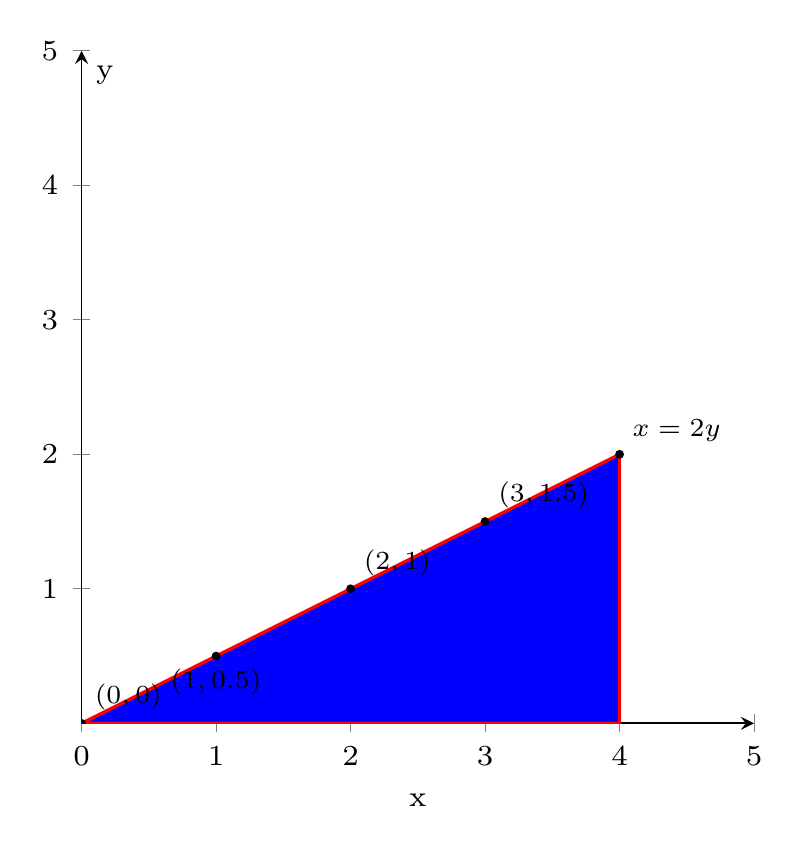
\begin{tikzpicture}[scale=1.5,line width=1pt]

\begin{axis}[
color= black,
xmin=0, 
xmax=5, 
ymin=0, 
ymax=5, 
axis equal image, 
axis x line=left,
axis y line=middle,
%xticklabels={}, 
%yticklabels={},
font=\scriptsize,
%ticks=none,
%extra x ticks=0,
%extra y ticks=0,
xlabel={x},
ylabel={y},
]

%\draw (0,675) -- (1000,0);
\addplot [thick, red,fill=blue,smooth] coordinates {(0,0) (1,0.5) (2,1) 
(3,1.5) (4,2)} \closedcycle;
%\draw [thick, red!20, fill=red!20] (0,0) -- (0,675) -- (1000,0) -- cycle;
\filldraw[black] (0,0) circle (0.03cm) node[above right, scale=0.9] 
{$(0,0)$};
\filldraw[black] (1,0.5) circle (0.03cm) node[below, scale=0.9] 
{$(1,0.5)$};
\filldraw[black] (2,1) circle (0.03cm) node[above right, scale=0.9] 
{$(2,1)$};
\filldraw[black] (3,1.5) circle (0.03cm) node[above right, scale=0.9] 
{$(3,1.5)$};
\filldraw[black] (4,2) circle (0.03cm) node[above right, scale=0.9] 
{$x=2y$};


\end{axis}

\end{tikzpicture}

\vspace{0.2cm}

\textbf{\underline{Part b}}: Finding P(X$>$Y, X$<$2Y)

\vspace{0.2cm}

From the graph below, we need to integrate the joint probability density over the orange area. For that, we will integrate over the complete X $>$ Y region and subtract the blue region (X $\geq$ 2Y) from it.

From equation 9, we already found the value under the blue region is $\frac{1}{4}$

\begin{equation} 
\begin{split}
P(X>Y ,X<2Y) & = \iint_A f_{XY}(x,y) dx dy \\
 & = \iint_A 1/16 dx dy \\
 & = \int_{0}^{4} \int_{0}^{x} \frac{1}{16} dy dx - \int_{0}^{4} \int_{0}^{x/2} \frac{1}{16} dy dx\\
 & = \int_{0}^{4} \frac{x}{16} dx - \int_{0}^{4} \frac{x}{32} dx  \\ 
 & = \frac{1}{2} - \frac{1}{4} = \frac{1}{4}
\end{split}
\end{equation}




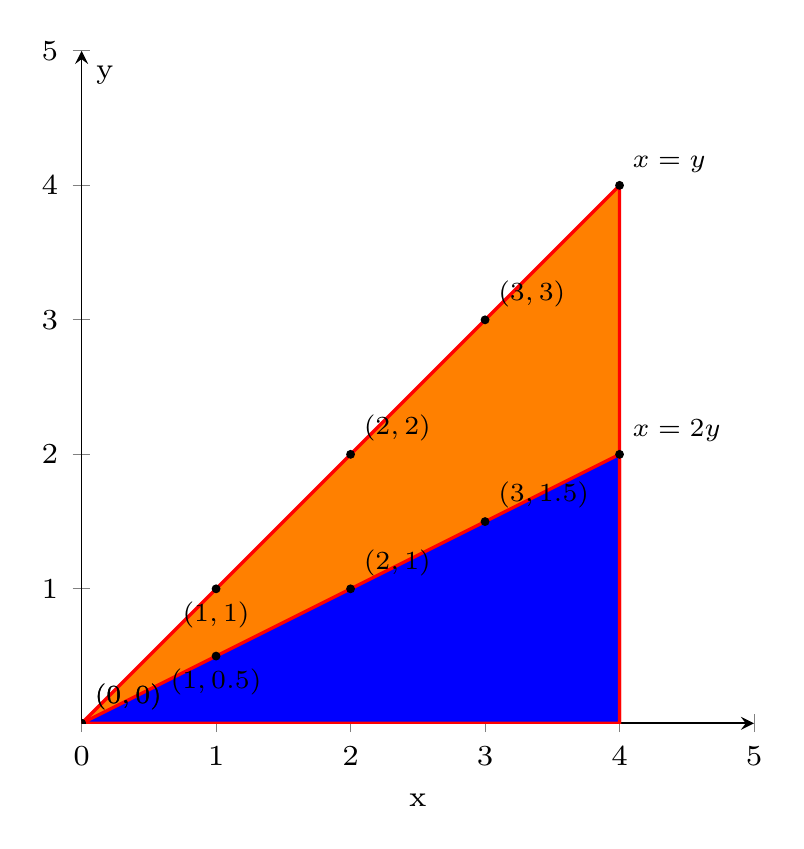
\begin{tikzpicture}[scale=1.5,line width=1pt]

\begin{axis}[
color= black,
xmin=0, 
xmax=5, 
ymin=0, 
ymax=5, 
axis equal image, 
axis x line=left,
axis y line=middle,
%xticklabels={}, 
%yticklabels={},
font=\scriptsize,
%ticks=none,
%extra x ticks=0,
%extra y ticks=0,
xlabel={x},
ylabel={y},
]

%\draw (0,675) -- (1000,0);
\addplot [thick, red,fill=orange,smooth] coordinates {(0,0) (1,1) (2,2) 
(3,3) (4,4)} \closedcycle;

\addplot [thick, red,fill=blue,smooth] coordinates {(0,0) (1,0.5) (2,1) 
(3,1.5) (4,2)} \closedcycle;

%\draw [thick, red!20, fill=red!20] (0,0) -- (0,675) -- (1000,0) -- cycle;
\filldraw[black] (0,0) circle (0.03cm) node[above right, scale=0.9] 
{$(0,0)$};
\filldraw[black] (1,0.5) circle (0.03cm) node[below, scale=0.9] 
{$(1,0.5)$};
\filldraw[black] (2,1) circle (0.03cm) node[above right, scale=0.9] 
{$(2,1)$};
\filldraw[black] (3,1.5) circle (0.03cm) node[above right, scale=0.9] 
{$(3,1.5)$};
\filldraw[black] (4,2) circle (0.03cm) node[above right, scale=0.9] 
{$x=2y$};

\filldraw[black] (0,0) circle (0.03cm) node[above right, scale=0.9] 
{$(0,0)$};
\filldraw[black] (1,1) circle (0.03cm) node[below, scale=0.9] 
{$(1,1)$};
\filldraw[black] (2,2) circle (0.03cm) node[above right, scale=0.9] 
{$(2,2)$};
\filldraw[black] (3,3) circle (0.03cm) node[above right, scale=0.9] 
{$(3,3)$};
\filldraw[black] (4,4) circle (0.03cm) node[above right, scale=0.9] 
{$x=y$};


\end{axis}

\end{tikzpicture}

\vspace{0.3cm}
Substitute results from (10) and (11) in  equation 2, 
 
 \begin{equation}
     \Rightarrow P(X>Y | X<2Y) = \frac{1/4}{3/4} = \frac{1}{3}
 \end{equation}
 

\end{document}
